


\paragraph{Scalatura.}Data una coppia $s(t) \fCouple S(f)$ allora:
\lezione{Lezione 12}{05/11/2024} 
\begin{equation}
    s(at) \fCouple \frac{1}{|a|}S\left(\frac{f}{a}\right)
\end{equation}

\paragraph{Dimostrazione}
Consideriamo $a > 0$:
\begin{equation*}
    \fourier\{s(at)\} = \int_{-\infty}^{+\infty}s(at)e^{-j2 \pi ft}dt
\end{equation*}
Ora consideriamo questo cambio di variabili $
    \begin{cases}
        \tau = at\\
        d\tau = adt
    \end{cases}
$

\begin{gather*}
    =\int_{-\infty}^{+\infty}s(at)e^{-j2 \pi ft}dt=\\
    =\int_{-\infty}^{+\infty}s(\tau)e^{-j2 \pi f\frac{\tau}{a}}\frac{d\tau}{a}=\\
    = \frac{1}{a} \int_{-\infty}^{+\infty}s(\tau)e^{-j2 \pi \frac{f}{a} \tau} \tau=\\
    = \frac{1}{a} S\left(\frac{f}{a}\right)
\end{gather*}

Poi in maniera simile, per $a < 0$ possiamo dimostrare che $\fourier\{s(at)\} = \frac{1}{-a} S\left(\frac{f}{a}\right)$.
Allora possiamo unificare i 2 risultati considerando la $a$ in valore assoluto.

\paragraph{Derivazione}
Data una coppia $s(t) \fCouple S(f)$ allora:
\begin{equation}
    \frac{d}{dt}s(t) \fCouple j2\pi f S(f)
\end{equation}
\paragraph{Dimostrazione}
\begin{gather*}
    \frac{d}{dt}s(t) =\\
    = \frac{d}{dt} \int_{-\infty}^{+\infty} S(f) e^{j2 \pi ft}df =\\ \tag{formula di Sintesi}
    = \int_{-\infty}^{+\infty} S(f) \frac{d}{dt} e^{j2 \pi ft} df =\\
    = \int_{-\infty}^{+\infty} S(f) j2\pi f e^{j2 \pi ft} df =\\
    =  \int_{-\infty}^{+\infty} [j2\pi f S(f)] e^{j2 \pi ft} df
\end{gather*}
Allora abbiamo trovato la coppia di fourier $\frac{d}{dt}s(t) \fCouple j2\pi f S(f)$

\paragraph{Convoluzione}
Date le seguenti coppie di Fourier $x(t) \fCouple X(f)$ e $y(t) \fCouple Y(f)$ allora:
\begin{equation}
    x(t) \ast y(t) \fCouple X(f)Y(f)
\end{equation}
\paragraph{Dimostrazione}
\begin{gather*}
    \fourier\{x(t) \ast y(t)\} = \\
    = \fourier\{\int_{-\infty}^{+\infty}x(\tau)y(t - \tau) d\tau\} =\\
    = \int_{-\infty}^{+\infty} \int_{-\infty}^{+\infty} x(\tau)y(t - \tau)d\tau e ^{-j2\pi ft} dt
\end{gather*}
Consideriamo ora $e ^{-j2\pi ft} = e ^{-j2\pi f(t - \tau +\tau)} = e ^{-j2\pi f(t - \tau)}e^{-j2\pi \tau} $
\begin{gather*}
    = \int_{-\infty}^{+\infty} \int_{-\infty}^{+\infty} x(\tau)y(t - \tau)e ^{-j2\pi f(t - \tau)}e^{-j2\pi \tau} d\tau  dt=\\
    = \int_{-\infty}^{+\infty} \int_{-\infty}^{+\infty} \{x(\tau)e^{-j2\pi \tau}  d\tau \} y(t - \tau) e ^{-j2\pi f(t - \tau)}  dt =\\
    = \int_{-\infty}^{+\infty} X(f) y(t - \tau) e ^{-j2\pi f(t - \tau)}  dt =\\
    = X(f)Y(f)
\end{gather*}
Per \textbf{Dualità} si ottiene anche che:
\begin{equation}
    x(t)y(t) \fCouple X(f) \ast Y(f)
\end{equation}

\paragraph{Integrazione}
Data la coppia di Fourier $s(t) \fCouple S(f)$ e data la funzione $p(t) = \int_{-\infty}^{t} s(\tau) d\tau$ allora:
\begin{equation}
    p(t) \fCouple \frac{1}{2j\pi f} S(f) + \underbrace{\frac{S(0)}{2}S(f)}_{\text{costante integrazione}}
\end{equation}

\newpage

\subsection{Teorema Di Parseval (Energia)}
Il teorema di Parseval per Segnali Energia (vedi paragrafo \ref{def: sep}) afferma che la trasformata di un segnale conserva
sempre l'energia, ossia:
\begin{equation}
    \int_{-\infty}^{+\infty} |s(t)|^2 dt = \int_{-\infty}^{+\infty} |S(f)|^2 df
\end{equation}

\paragraph{Dimostrazione}
\begin{align*}
    &\int_{-\infty}^{+\infty} |s(t)|^2 dt = \\
    = &\int_{-\infty}^{+\infty} s(t) \overline{s(t)} dt= \\ \tag{per eq. di Sintesi}
    = &\int_{-\infty}^{+\infty} \overline{s(t)} \left[\int_{-\infty}^{+\infty} S(f) e^{j2 \pi ft}df \right] dt =\\
    = &\int_{-\infty}^{+\infty} S(f)  \left[\int_{-\infty}^{+\infty} \overline{s(t)}e^{j2 \pi ft}dt \right] df =\\
\end{align*}
Sfruttiamo ora la seguente proprietà: $a \cdot b = \overline{\overline{a} \cdot \overline{b}}$:
\begin{align*}
    = &\int_{-\infty}^{+\infty} S(f)  \left[\int_{-\infty}^{+\infty} \overline{s(t)}e^{j2 \pi ft}dt \right] df = \\
    = &\int_{-\infty}^{+\infty} S(f)  \overline{\int_{-\infty}^{+\infty} s(t) e^{-j2 \pi ft}}dt df = \\
    = &\int_{-\infty}^{+\infty} S(f) \overline{S(f)} df =\\
    = &\int_{-\infty}^{+\infty} |S(f)|^2df 
\end{align*}
Intuitivamente, possiamo dire che, l'energia di un segnale è proprio uguale alla somma dell'energia trasportata da ogni
contributo dei seni a tutte le frequenze della trasformata. Proprio per questo motivo $|S(f)|^2$ viene anche detta \textbf{Densità
Spettrale di Energia}

\subsection{Teorema di Parseval (Potenza)} 

Similmente al Teorema per i segnali energia, ne esiste uno simile per i segnali potenza:
\begin{equation}
    \lim_{T \to +\infty} \frac{1}{2T} \int_{-T}^{+T} |s(t)|^2 dt = \int_{-\infty}^{+\infty} |S(f)|^2df
\end{equation}
$|S(f)|^2$ viene anche detta \textbf{Densità spettrale di frequenza}


\subsection{Sistemi nel Dominio delle Frequenze}
Abbiamo visto che, per la proprietà fondamentale dei sistemi LTI \eqref{prop: fondLTI}, l'output di un sistema
può essere visto come il risultato della convoluzione tra l'input e la risposta all'impulso. Per la proprità 
commutativa della convoluzione abbiamo scoperto che è vero anche il contrario, è possibile studiare un sistema 
studiando la risposta all'ingresso, che è un segnale. Per questo motivo ha senso estendere l'analisi in Frequenza
anche per i Sistemi LTI.

Ricordando la proprietà di risposta all'impulso \eqref{prop: rispInFreq}, possiamo dire che $H(f)$ sia a tutti
gli effetti la trasformata di Fourier della risposta all'impulso e può essere vista come risposta ad un Fasore.
Cerchiamo di definire uno schema generale dei sistemi LTI nel dominio delle frequenze e del tempo:
\begin{center}
    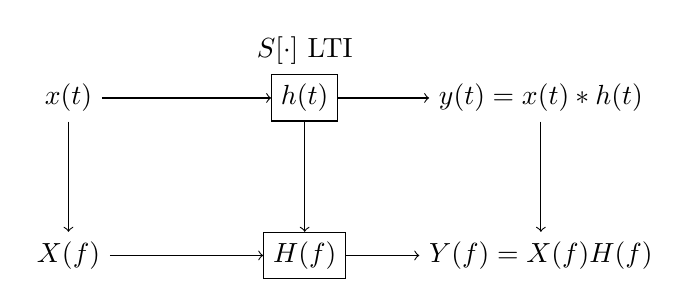
\begin{tikzpicture}

        % Nodi della prima fila
        \node (A1) at (-3, 0) {$x(t)$};
        \node[rectangle, draw] (B1) at (0,0) {$h(t)$};
        \node (T) at (0,0.6) {{$S[\cdot]$ LTI}};
        \node (C1) at (3,0) {$y(t) = x(t) \ast h(t)$};
    
        % Nodi della seconda fila
        \node (A2) at (-3,-2) {$X(f)$};
        \node[rectangle, draw] (B2) at (0,-2) {$H(f)$};
        \node (C2) at (3,-2) {$Y(f) = X(f)H(f)$};
    
        % Frecce dal primo livello al secondo
        \draw[->] (A1) -- (B1) ;
        \draw[->] (B1) -- (C1)  ;
        \draw[->] (A1) -- (A2) node[midway, left] {$\fourier$};
        \draw[->] (B1) -- (B2) node[midway, left] {$\fourier$};
        \draw[->] (C1) -- (C2) node[midway, left] {$\fourier$};
        \draw[->] (A2) -- (B2)  ;
        \draw[->] (B2) -- (C2) ;
    
    \end{tikzpicture}
\end{center}

L'analisi in frequenza di un sistema è importantissimo per 2 grandi proprietà:
\begin{itemize}
    \item Dal momento che $Y(f) = X(f)H(f)$, possiamo dire che per ogni frequenza $f$, la risposta in frequenza $H(f)$
    amplifica, diminuisce, o annulla l'ampiezza dell'ingresso $X(f)$, tuttavia $Y(f)$ continua ad essere un fasore con la stessa frequenza dell'ingresso.
    Possiamo dunque dire che $H(f)$ agisce da \textbf{Filtro} per le frequenze che compongono l'ingresso $x(t)$.
    \item Dal punto di vista di \textbf{calcolo numerico}, calcolare per tutti gli istanti la convoluzione di $x(t) \ast h(t)$ non è proprio semplice;
    Grazie all'analisi in frequenza, però, possiamo fare un'escamotage: calcolare le 2 trasformate, moltiplicarle e antitrasformarle. Operazione di gran
    lunga più semplice che calcolare la convoluzione.
\end{itemize}
Dall'analisi in frequenza di un sistema notiamo che:
\begin{itemize}
    \item $|Y(f)| = |X(f)||H(f)|$
    \item $\angle Y(f) = \angle X(f) + \angle H(f)$
\end{itemize}